\documentclass[english,a4paper,twoside]{scrreprt}

% Used packages
\usepackage[printonlyused]{acronym}
\usepackage{amsfonts}
\usepackage{amsmath}
\usepackage{amssymb}
\usepackage{babel}
\usepackage{calc}
\usepackage{chngpage}
\usepackage{fancyhdr}
\usepackage{graphicx}
\usepackage{listings}
\usepackage{url}
\usepackage{color}
\usepackage[pdftex,%
    pdfpagemode={UseOutlines},%
    bookmarks,%
    colorlinks,%
    linkcolor={blue},%
    plainpages=false,%
    pdfpagelabels,%
    citecolor={red}]{hyperref}

\newcommand{\Rvk}{Reykjav\'\i{}k }

% Global settings.
\setlength{\parskip}{\medskipamount}
\setlength{\parindent}{0pt}
\setlength{\textheight}{22cm}

% Listing settings.
\lstset{basicstyle=\fontfamily{cmss}\small,frame=tb}
\lstset{columns=fixed,basewidth=0.5em,keepspaces=true}
\lstset{aboveskip=1em,belowskip=0.5em}
\lstset{numbers=left,numberstyle=\tiny,stepnumber=5}
\lstset{showtabs=false,showspaces=false,showstringspaces=false}

% Improved title page.
\makeatletter
\newcommand{\institution}{\newcommand{\@institution}}
\renewcommand\maketitle{\begin{titlepage}%
\let\footnotesize\small
\let\footnoterule\relax
\let \footnote \thanks
\null\vfil
\vskip 60\p@
\begin{center}%
  {\LARGE \@title \par}%
  \vskip 3em%
  {\large
   \lineskip .75em%
    \begin{tabular}[t]{c}%
      \@author
    \end{tabular}\par}%
    \vskip 1.5em%
  {\large \@date \par}%       % Set date in \large size.
\end{center}\par
\@thanks
\vfill
{\small
 \begin{flushright}
  \begin{tabular}{l}\hline
  \@institution\hline
  \end{tabular}
 \end{flushright}
}
\global\let\@institution\@empty
\global\let\institution\relax
\end{titlepage}
}

% Improved acronym environment.
\newenvironment{acronym*}[1]{%
   \newcommand{\acrolabel}[1]{\textbf{##1}\hfil}%
   \providecommand*{\acro}{\AC@acro}%
   \begin{list}{}{%
      \renewcommand{\makelabel}{\acrolabel}%
      \settowidth{\labelwidth}{\textbf{#1}}%
      \setlength{\leftmargin}{\labelwidth+\labelsep}%
      }
   }{%
   \end{list}
}\makeatother

% Fancy header settings.
\pagestyle{fancy}
\renewcommand{\chaptermark}[1]{\markboth{#1}{}}
\renewcommand{\sectionmark}[1]{\markright{\thesection\ #1}}
\fancyhf{}
\fancyheadoffset[LE,RO]{\marginparsep+\marginparwidth}
\fancyhead[LE,RO]{\bfseries\thepage}
\fancyhead[LO]{\bfseries\rightmark}
\fancyhead[RE]{\bfseries\leftmark}
\fancypagestyle{plain}{%
  \fancyhead{}\renewcommand{\headrulewidth}{0pt}}

% Document meta data.
%FIXME: better title & remove draft suffix
\title{Ambient Earth\\
       {\Large \emph{Internship report --- 1$^{\text{st}}$ draft\/}}}
\author{Christian Luijten\\\url{christian06@ru.is}}
\date{\today}
\institution{
 CADIA group \\
 School of Science and Engineering \\
 \Rvk University, \Rvk \\[1em]
 \emph{Under supervision of:\/} \\
 Kristinn R. Th\'orisson, Ph.D. (\Rvk University) \\
 dr.ir. Huub van de Wetering (Eindhoven University of Technology) \\
}

\begin{document}

\acrodef{RU}{\Rvk University}
\acrodef{TU/e}{Technical University Eindhoven}
\acrodef{CADIA}{Center for Analysis \& Design of Intelligent Agents}

\maketitle

\mbox{} \\
\vfill

\begin{adjustwidth}{4em}{4em}
{\scriptsize
  Christian Luijten (\url{christian06@ru.is})

  Copyright \copyright\ 2006 Center for Analysis and Design of Intelligent
  Agents. \\
  \Rvk{} University \\
  All rights reserved

  \url{http://cadia.ru.is/}

  Redistribution and use in source and binary forms, with or without
  modification, is permitted provided that the following conditions are met:

  \begin{itemize}
    \item Redistributions of source code must retain the above copyright
      notice, this list of conditions and the following disclaimer.

    \item Redistributions in binary form must reproduce the above copyright
      notice, this list of conditions and the following disclaimer in the
      documentation and/or other materials provided with the distribution.

    \item Neither the name of its copyright holders nor the names of its
      contributors may be used to endorse or promote products derived from this
      software without specific prior written permission.

  \end{itemize}

  THIS SOFTWARE IS PROVIDED BY THE COPYRIGHT HOLDERS AND CONTRIBUTORS "AS IS"
  AND ANY EXPRESS OR IMPLIED WARRANTIES, INCLUDING, BUT NOT LIMITED TO, THE
  IMPLIED WARRANTIES OF MERCHANTABILITY AND FITNESS FOR A PARTICULAR PURPOSE
  ARE DISCLAIMED. IN NO EVENT SHALL THE COPYRIGHT OWNER OR CONTRIBUTORS BE
  LIABLE FOR ANY DIRECT, INDIRECT, INCIDENTAL, SPECIAL, EXEMPLARY, OR
  CONSEQUENTIAL DAMAGES (INCLUDING, BUT NOT LIMITED TO, PROCUREMENT OF
  SUBSTITUTE GOODS OR SERVICES; LOSS OF USE, DATA, OR PROFITS; OR BUSINESS
  INTERRUPTION) HOWEVER CAUSED AND ON ANY THEORY OF LIABILITY, WHETHER IN
  CONTRACT, STRICT LIABILITY, OR TORT (INCLUDING NEGLIGENCE OR OTHERWISE)
  ARISING IN ANY WAY OUT OF THE USE OF THIS SOFTWARE, EVEN IF ADVISED OF THE
  POSSIBILITY OF SUCH DAMAGE.
}
\end{adjustwidth}

\tableofcontents

\addcontentsline{toc}{chapter}{Preface \& Acknowledgements}
\chapter*{Preface \& Acknowledgements}

During the period of September to November 2006 I have been working at the
\ac{CADIA} research lab of the School of Science and Engineering of the \ac{RU}
in Iceland.

I would like to thank Kristinn Th\'orisson of \ac{RU} for giving me this
opportunity.

When I considered doing part of my studies abroad, there was no agreeement with
any Icelandic institution yet. I had thought of an internship at a Scandinavian
university and by coincidence I discovered that just weeks before an agreement
was signed between \ac{TU/e} and \ac{RU}. 

Since Iceland was high on my ``wish to visit once'' list, this was a perfect
chance. From this position I would therefore also like to thank Jan-Friso
Groote (\ac{TU/e}) and Luca Aceto (\ac{RU}) for initiating this agreement.

Others who made my stay a pleasant one were the people from the International
Offices of \ac{RU} and the University of Iceland, my fellow students both at
\ac{CADIA} and the Erasmus Intensive Language Course in August.

I have never experienced anything like this before.

Thank you very much!


\chapter{\label{cpt:introduction}Introduction}

This document describes the activities concerning my internship at \Rvk{}
University. The introduction, which you are reading right now, describes the
structure of this document.

Chapter~\ref{cpt:assignment} describes the initial assignment as given by
Kristinn R.  Thorisson of \Rvk{} University. Since the final product differs
from this first idea, the changes and their reasoning are given.

In Chapter~\ref{cpt:planning} a planning is proposed. It is taken from the
planning as written in the logbook which I held online at
\url{http://nemendur.ru.is/christian06/logbook.html}.

The design of the system to be built is given in Chapters~\ref{cpt:scenarios},
\ref{cpt:requirements}, and \ref{cpt:architecture}. These chapters are included
from the design document. The full document can be downloaded from
\url{http://nemendur.ru.is/christian06/amber/design.pdf} or the most recent
version can be requested directly from the author, preferably by E-mail.

The complete internship is evaluated in Chapter~\ref{cpt:evaluation}. This will
contain learning points, which aspects went according to expectations and what
can be improved.

The document itself is concluded in Chapter~\ref{cpt:conclusion}.



\chapter{\label{cpt:assignment}Assignment}

The original assignment as written down by Kristinn Thorisson:

\begin{quote}

  The ``Semantic Ambient Web Monitor'' project's goal is to give people a sense
  of online acitivity and community interest regarding particular topics of
  interest and discussion. The prototype will have a simple small area where
  elements related to online activity -- each dot representing e.g. a posting
  on an online forum or a blog site about the particular topic of interest.
  Each corner represent a concept related to the topic; If the topic to be
  monitored is ``artificial intelligence'', one corner might represent
  ``humanoid robots'', another might represent ``artificial neural networks'',
  a third could be ``expert systems'' and a fourth could be ``machine
  learning''. As the dots move they get pulled stronger towards the center the
  older they are; the more they relate to a concept the closer they get pulled
  towards the corner representing that concept.

  This produces very ``holistic'' patterns that can be interpreted in an
  instant by an onlooker: An equal distribution of dots would mean that all
  concepts are discussed equally, on average, in all postings. An oval orbit
  would mean that the majority of postings are about the concepts in oposite
  corners of the square, etc. If the dots left trails one could see how things
  change over time, e.g. days or months. Snapshots of the square, e.g. one per
  day or month, would give you a visual history of how the disucssion has
  changed over time regarding those concepts.

  The methodology that will be used to build the monitor enables a very
  incremental, modular approach. The software will be made open-source and thus
  others can build monitors for other topics than those chosen in this project.

\end{quote}



\chapter{\label{cpt:planning}Planning}

The actual internship period amounts to 14 weeks and starts week 34. Before the
actual working period has started, the assignment was already largely agreed
upon.

A week by week planning and logbook was held during the internship at the web
address \url{http://nemendur.ru.is/christian06/logbook.html}.

\section{Week 34 and 35}

Learning the organization, methodologies and procedures.

\section{Week 36}

Having a global design of the modules and a first bit of object model,
meanwhile playing around with posting and retrieving messages with Psyclone.

\section{Week 37}

Finish global design, Think about visualization issues

\section{Week 38}

Create detailed design, code along, starting with basic visualization

\section{Week 39}

Create detailed design and code for crawler module. 

\section{Week 40}

Create detailed design and code for analysis modules.

\section{Week 41}

Continue detailed design and code for analysis modules.

\section{Week 42}

Continue detailed design and code for visualization. By the end of the week,
the EarthView widget should be finished so that in the next week the
communication with Psyclone can be created.

\section{Week 43}

Continue detailed design and code for visualization. Enable communication of
visualizer with Psyclone. By the end of the week, the applet should respond on
new stories and incoming analyses.

\section{Week 44}

Complete work at OpenGL visualization, return to crawler and sieves to use
parameter framework of Psyclone instead of own implementation.

\section{Week 45}

Refactoring, fixing bugs, completing Javadoc code documentation.

\section{Week 46}

Fine-tune crawling, analysis and visualization parameters. Create final
distribution files. Test those on various platforms.

\section{Week 47}

Finish everything up. No more coding this week! Reserved for ``Goodbyes''.

\section{Week 48}

Finish internship report and paperworks.




\chapter{\label{cpt:scenarios}Usage scenarios}

\section{A story is posted to a weblog}

When a story is posted on a weblog, it will show up in its RSS feed (this
happens of course outside of our responsibility). If \Amber\ is monitoring this
particular weblog, it will retrieve the story and analyze it. The story is then
displayed on a screen using the results of the analysis.

To get a more concrete idea, suppose \Amber\ is monitoring various A.I. related
weblogs and we would like to find out what they are mainly writing about. We
configure the analysis component in such a way that it can decide whether a
certain subject is dealt with in a story, thereby creating a profile for every
story. Stories with similar subjects will then show up close to eachother in
the display, stories with orthogonal subjects will be very far apart.

The result is an image with various ``clouds'' of in some way related stories.

\section{A discussion is held on a web forum}

Discussions on web forums can get lengthy and the main subject can change
multiple times during their lives. To get an idea what subjects the whole
discussion has been about, \Amber\ can show a cloud map of (part of) the
discussion. It could even show an animation to show how the discussion
developed over time.

Using the animated view of the discussion development, a new participant in the
discussion can decide upon whether bringing up an old discussion point is a
good idea or not. It is also a way to locate a certain subject within a long
list of replies.



\chapter{\label{cpt:requirements}Requirements}

There are various kinds of requirements to be identified. A distinction can be
made between functional and extra-functional (or non-functional) requirements.

\section{Extra-functional requirements}

\begin{enumerate}
  \item The system must make use of the Psyclone framework for communication.
  \item The system will be implemented in the Java programming language.
  \item The display module with the Java Applet must be able to run on any
    machine with a properly installed and recent Java Virtual Machine (i.e.
    not only on the machine running the rest of the system).
  \item It must be possible to add modules with similar functionality to
    operate in parallel with modules already there. For example when the Java
    Applet is running, it should also be possible to have the full screen
    module running at the same time. 
\end{enumerate}

\section{Functional requirements}

These requirements describe which \emph{inputs}, \emph{outputs}, \emph{storage}
and \emph{computations} exist in the system and how they are \emph{timed and
synchronized}. Finally, since this is a very important part of the project,
there are two separate sections on \emph{story analysis} and
\emph{visualization} requirements.

\subsection{Inputs}

\begin{enumerate}
  \item The system must be configurable to specify which sources will be
        monitored.
  \item The system will use the configuration to get information from the
        internet from the specified sources.
  \item Configuration of the system goes via Psyclone using module parameters.
  % \item The display may have a set of controls to navigate through the
  % history of a feed.
  \item Parts of the system must accept triggers from Psyclone whiteboards.
  \item Sources must be \ac{RSS} feeds, possibly aggregated via an \ac{OPML}
    file. The system should however be prepared to support other source types
    as well (i.e. it should be easily expandable).
  \item The Applet display is non-interactive (no input).
\end{enumerate}

\subsection{Outputs}

\begin{enumerate}
  \item There is an output module which is to be used within a website,
        i.e. a Java Applet.
  \item There is an output module which runs standalone and in full screen
        and displays more information than the Applet can.
\end{enumerate}

\subsection{Storage}

\begin{enumerate}
  \item The system on itself does not store anything.
\end{enumerate}

\subsection{Computations}

\begin{enumerate}
  \item The system must decide of a delivered story what its subject(s) is/are.
  \item The system may put weights on the subjects instead of a boolean value.
\end{enumerate}

\subsection{Timing and synchronization}

Synchronization between modules is handled by Psyclone, so no requirements need
to be added to the system itself.

\subsection{Story analysis}

\begin{enumerate}
  \item When stories come in, they are analysed by analysis modules.
  \item Every module adds some meta-information to the story depending on the
    module analysis.
\end{enumerate}

\subsection{Visualization}

The following requirements are common for both the applet and the standalone
viewer.

\begin{enumerate}
  \item A story is represented as a dot.
  \item In the center of the display is Earth (with picture?).
  \item Dots are launched into orbit around Earth.
  \item The dots leave fading trails as they move.
  \item There are some small, heavy bodies in ``geostationary'' orbit around
    Earth representing values of an enumeration of meta-information (for
    instance story subjects). They attract the stories depending on how much
    they match the story's subject. 
\end{enumerate}

There will be two different views, a static and a dynamic one. Which one is
used depends on the application. To get an idea of the activity at a certain
moment in time, the static view is used. For a ``real-time'' view of internet
activity, the dynamic view can be used.

The term ``static'' doesn't mean the image is standing still, it will behave
exactly the same as the dynamic view. However, some physical laws don't apply
or are differently calibrated in order to give a constant image. In other
words, while in dynamic view stories can appear and disappear, in the static
view the stories are a given constant.

\subsubsection{Differences between Applet and Standalone viewer}

\begin{enumerate}
  \item The applet display will in practice be considerably smaller than the
    standalone viewer. Therefore, the applet is less detailed and some physical
    laws might need to be bend a bit.
\end{enumerate}



\chapter{\label{cpt:architecture}Architecture}

The architecture of \Amber\ is defined in terms of modules, whiteboards and the
messages they use to communicate. Figure~\ref{fig:global-architecture} shows
the flow of messages between the modules and whiteboards.

In the Section~\ref{sct:modules} the modules are described and in
Section~\ref{sct:messages} the messages connecting them are defined. % The data
% types used in the system are described in Section~\ref{sct:types}.

\begin{figure}
    \centering
    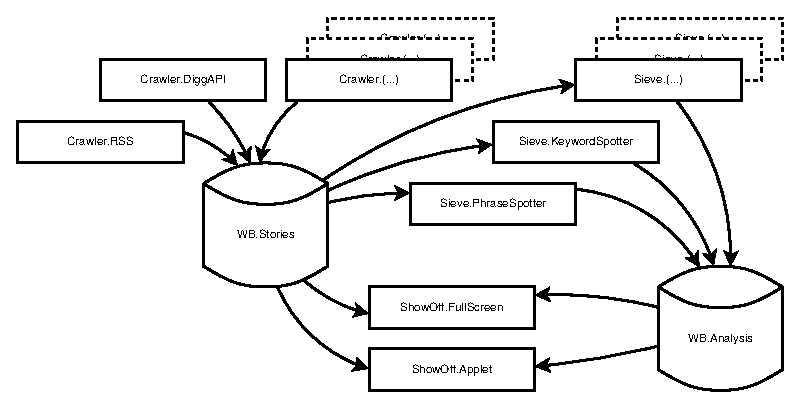
\includegraphics{\designpath/image/global-architecture}
    \caption{\label{fig:global-architecture}Global \Amber\ architecture, the
              names are Psyclone module names}
\end{figure}

\section{\label{sct:modules}Modules}

A complete \Amber\ system will comprise at least three modules running at the
same time; there is a Crawler module, a selector module called Sieve and a
display called ShowOff. The modules are separate executables with their own
life-cycles and resources. Since TCP/IP is used, the executables don't need to
be on the same machine to communicate.

Every module has a specified interface through which communication with
Psyclone is handled.

\subsection{Crawler modules}

When the Crawler is started, it will create one of the available handlers
(depending on what is specified on the command line or what is set as default
during build time). 

It also creates an AirBrush instance to communicate with Psyclone via
Java\-Open\-AIR. The module name announced to Psyclone is `Crawler.' plus the
name of the handler, so `Crawler.RSS' in case of the RSS handler.

After connecting with Psyclone, the handler can get its parameters stored in
the psySpec file and go to work. It will post stories with type `Story'  on the
whiteboard `WB.Stories'.

\subsubsection{RSS}

The RSS crawler module will be fairly straightforward. There are actually quite
a few good RSS parsers around for Java, the only thing the crawler should do is
getting the stories from the RSS feeds along with meta-information and store it
on the whiteboard.

Although the module is called RSS, it can also handle Atom feeds, which is also
quite a popular format.

\begin{module}{Crawler.RSS}
  \trigger{Feed.*}{WB.Control}
  \post{Story}{WB.Stories}
\end{module}

\subsubsection{DiggAPI}

Digg is a website which lets users submit stories found on the web. Other users
then moderate the submissions either by `digging' or `burying' a story. A story
with a lot of `diggs' is a popular one. The nice thing about Digg is that it
actually does a lot of preprocessing work for the \Amber\ system.

Digg
announced\footnote{\url{http://diggtheblog.blogspot.com/2006/07/digg-labs-launches-alpha.html}}
that they will publish a public API within the next months. If time allows, a
DiggAPI module is created.

\begin{module}{Crawler.DiggAPI}
    \post{Story}{WB.Stories}
\end{module}

% \subsubsection{BloggerDataAPI}
% 
% One of the larger weblog hosters is Google with their Blogger service. There
% is an API available to get information from it.
% 
% \begin{module}{Crawler.BloggerDataAPI}
%   \post{Story}{WB.Stories}
% \end{module}


\subsection{Sieve modules}

All analysis modules, or sieves, will get a trigger from a new story on the
whiteboard WB.Stories. They analyse it and if there is anything to say about
the story, a Analysis message is sent to the whiteboard WB.Analyses containing
its judgement on the story.

The contents of this message is specified in Section~\ref{sct:messages}.

Analysis modules may take any time they like to come to a verdict, but it is
possible that a story has already disappeared from the visualization if the
response is very late.

Since all modules employ the same external behaviour, the Psyclone
specification is the same for every one of them.

\begin{module}{Sieve.???}
    \trigger{Story}{WB.Stories}
    \post{Analysis}{WB.Analyses}
\end{module}

\subsection{ShowOff modules}

The ShowOff modules are visualizers which combine the crawled stories from the
Crawler with the analyses from the Sieve modules.

\begin{module}{ShowOff.???}
    \trigger{Story}{WB.Stories}
    \trigger{Analysis}{WB.Analyses}
\end{module}

\subsubsection{Full screen}

The full screen application will display a lot of information and is there to
be looked - not glanced - at. It should be possible to let it do its job
autonomously, just showing a pretty picture, or to be interactive.

\subsubsection{Ambient applet}

The ambient applet will display a very easy to understand image (a glance at it
should be enough) of the status of the page it is on. I.e. if the page is a
weblog, it should display subject information on that weblog, if it is on the
page of a thread of a forum, it displays the flow of the discussion.



\section{\label{sct:messages}Messages}

There are a few message types in the system. Two of which must be defined
system-wide because they are used in the communication between modules.

\subsection{\label{sct:messages:story}Message type `Story'}

The Story message is only posted to the whiteboard `WB.Stories' and only by
Crawler modules.

The message content is a \ac{YAML}\footnote{\url{http://www.yaml.org/}} document
which represents the storyData field inside the Java counterpart of the
message. It contains at least the properties `URI' (to identify the story,
GUIDs are RSS specific and cannot be used), `Author', `Title', `Story-Content'.

It may also contain `Publication-Date' (which is the date of publication in
Internet~Message~Format\cite[Section~3.3]{RFC2822}), `Kind' and other fields.

An example of a YAML document containing Story data:

\begin{verbatim}
---
URI: http://ijsland.luijten.org/2006/09/12/skyr-wasdanou/
Author: Christian Luijten
Title: Skyr... Wasdanou?
Publication-Date: Tue, 12 Sep 2006 21:03:54 +0000
Kind: weblog-posting
Story-Content: >
  Een van die dingen die bij een onbekende cultuur horen zijn de
  eetgewoonten. Elk land heeft zo z’n producten die je nergens
  anders kan krijgen. IJslands nationale zuivelproduct heet Skyr,
  elke oma kan het maken, al is het nogal een hoop werk. Daarom is
  het lange tijd (lees: gedurende de jachtige periode na de tweede
  wereldoorlog toen de Amerikanen hier de boel kwamen ophaasten)
  in ongebruik geraakt, maar op een gegeven moment kwam de vraag
  toch weer terug en zijn een aantal zuivelproducenten het
  industrieel gaan produceren.
\end{verbatim}

\subsection{Message type `Analysis'}

Analysis typed messages are posted on the `WB.Analysis' whiteboard only by
Sieve modules. They contain information about stories present on the
`WB.Stories' whiteboard.

The content of these messages is also YAML format. Stories and Analysis
messages are coupled through their `URI' fields, so this must be present.

An example of a message issued by an analysis module checking for the topic
`Zuivel' (which means dairy products in Dutch):

\begin{verbatim}
---
URI: http://ijsland.luijten.org/2006/09/12/skyr-wasdanou/
Topic: Zuivel
Relation-Strength: 1.0
Author-Strength: 0.1
\end{verbatim}

Its `Relation-Strength' suggests high relevance of the content with the topic.
However, the `Author-Strength' suggests that the author isn't an authority in
the field.

Every analysis module sends a message to the whiteboard if it thinks it is
relevant. It is thus possible that the same URI will get multiple analysis
results or nothing at all, the visualizer module must cope with this and merge
the available information.



% \input{\designpath/04.3-types.inc}



\chapter{Detailed design}

The fully documented source code with detailed design can be found in the
design document which is available at
\url{http://nemendur.ru.is/christian06/amber/design.pdf} or directly from the
author.



\chapter{\label{cpt:evaluation}Evaluation}

\section{Educational evaluation}

\subsection{Learning points}

The approach used in the development of this project is called
Constructionists Design Methodology, which is a form of incremental
design. For this project, this was a good choice, because many things were
undecided upon in the beginning and only became clear after some first
experiments.

One example would be the visualization of ``replies to a story'' which was
initially thought of as adding a particle on a tail tied to the original
story. The longer the tail, the more important a story would appear.

However, there is no connection between a reply and a story other than a
humanly constructed one (there is no field in RSS which specifies it). It
was thus impossible to create this link without going far beyond the scope
of this project.

Instead, it was chosen to give all replies their own orbiting particles
and if a story is popular, many particles appear and in this way visualize
activity in a topic.

\subsection{Points for improvement}

It is very hard to create a realistic planning and to estimate one's
capabilities right. Some details had to be simplified on the way to make
the project fit within the available time, while other aspects which
seemed complex were in fact solved very quickly.

\section{Technical evaluation}

\subsection{Unimplemented parts}

It is not yet possible to ``travel through the past'' as was an initial
idea. This feature would enable a user to set a certain time in the past
and see the situation at that point. A very simple approach would be to
create screenshots of the display for every day and then display the
desired one.

\subsection{Points for expansion}

The nice thing about using a message and whiteboarding system like
Psyclone is that every component can be replaced fairly easily.

Currently, there is only one analysis module which can not make very
intelligent decisions. The fact that this is a project within the AI
department, makes it likely that someone will implement a smarter analysis
module which can run in place or alongside the current one.

It is only possible to get stories from RSS feeds, but another module
could be created which gets information out of newsgroups. A lot of
AI discussion is going on on Usenet, so this might also be an interesting
expansion of the system.

If the applet is to be used in a forum, it can be that a module with
direct (read-only) database access is created.

Then, finally, the visualization itself can be replaced by another one and
one of the ideas is to make it look more like the Sun's corona, expanding
it in those directions where much discussion is going on, shrinking it
where discussion is quiet.


\chapter{\label{cpt:conclusion}Conclusion}




% \appendix

% \input{app_plain_grammar.tex.inc}

% \input{app_xml_dtd.tex.inc}

% \input{app_examples.tex.inc}

% \input{app_impl_output.tex.inc}

\addcontentsline{toc}{chapter}{\refname}
% \bibliographystyle{cadia}
% \bibliography{cadia,additional}

\end{document}
